\documentclass[11pt,a4paper]{article}
\usepackage[margin=22mm]{geometry}
\usepackage[T1]{fontenc}
\usepackage{lmodern,tabularx,booktabs,hyperref,xcolor,graphicx,array}
\setlength{\parindent}{0pt}
\setlength{\parskip}{6pt}

\title{Design Pattern Analysis in a Vue.js-Based Social Media Application}
\author{Team A13: Sreehari M; Rohit Prasanth; Sreyas S Sankar; Sreevisakh A; Vighnesh H}
\date{2026-10-12}

\begin{document}
\maketitle

Team A13. Students: AM.SC.U4CSE23156 Sreehari M; AM.SC.U4CSE23148 Rohit Prasanth; AM.SC.U4CSE23157 Sreyas S Sankar; AM.SC.U4CSE23173 Sreevisakh A; AM.SC.U4CSE23168 Vighnesh H. Batch: CSE B (all members).

Case study: Design Pattern Analysis in a Vue.js-Based Social Media Application. Application: Misskey (https://github.com/misskey-dev/misskey), licence GNU AGPL-3.0, baseline commit 5f501341d49d2bc3fa7e817ce7548a82174326eb (version 2026.10.0). Repository folder: A13 in the 23CSE455 case-study repository.

\section{Application and architecture}
Misskey is an open-source federated social media platform. Its frontend is a Vue 3 application (Vue 3.5.42) and its backend is a NestJS application (NestJS 11.2.3) using TypeORM repositories, Redis, BullMQ job queues and Fastify routes. The analysis covers the code under packages/backend, packages/frontend and packages/misskey-js that the pattern records cite; everything else was not examined in depth.

Environment of the Part 3 measurements: OpenJDK 17.0.19, CPython 3.14.6, Node.js v24.15.0, g++ 16.1.1 (-std=c++17), lizard 1.24.1, on one Linux x86\_64 laptop (Intel i7-9750H). Part 2 tests ran with the repository unit-test runner (vitest) against in-memory doubles because PostgreSQL and Redis were not available.

Run instructions: each Part 3 snippet folder has a README with its test command (example: python3 -B test\_logging\_factory.py ../../../test-cases/factory.txt from Part3/code/pattern\_factory/python/). Part 2 commands and logs are in Part2/changes/Change1-4.

\begin{center}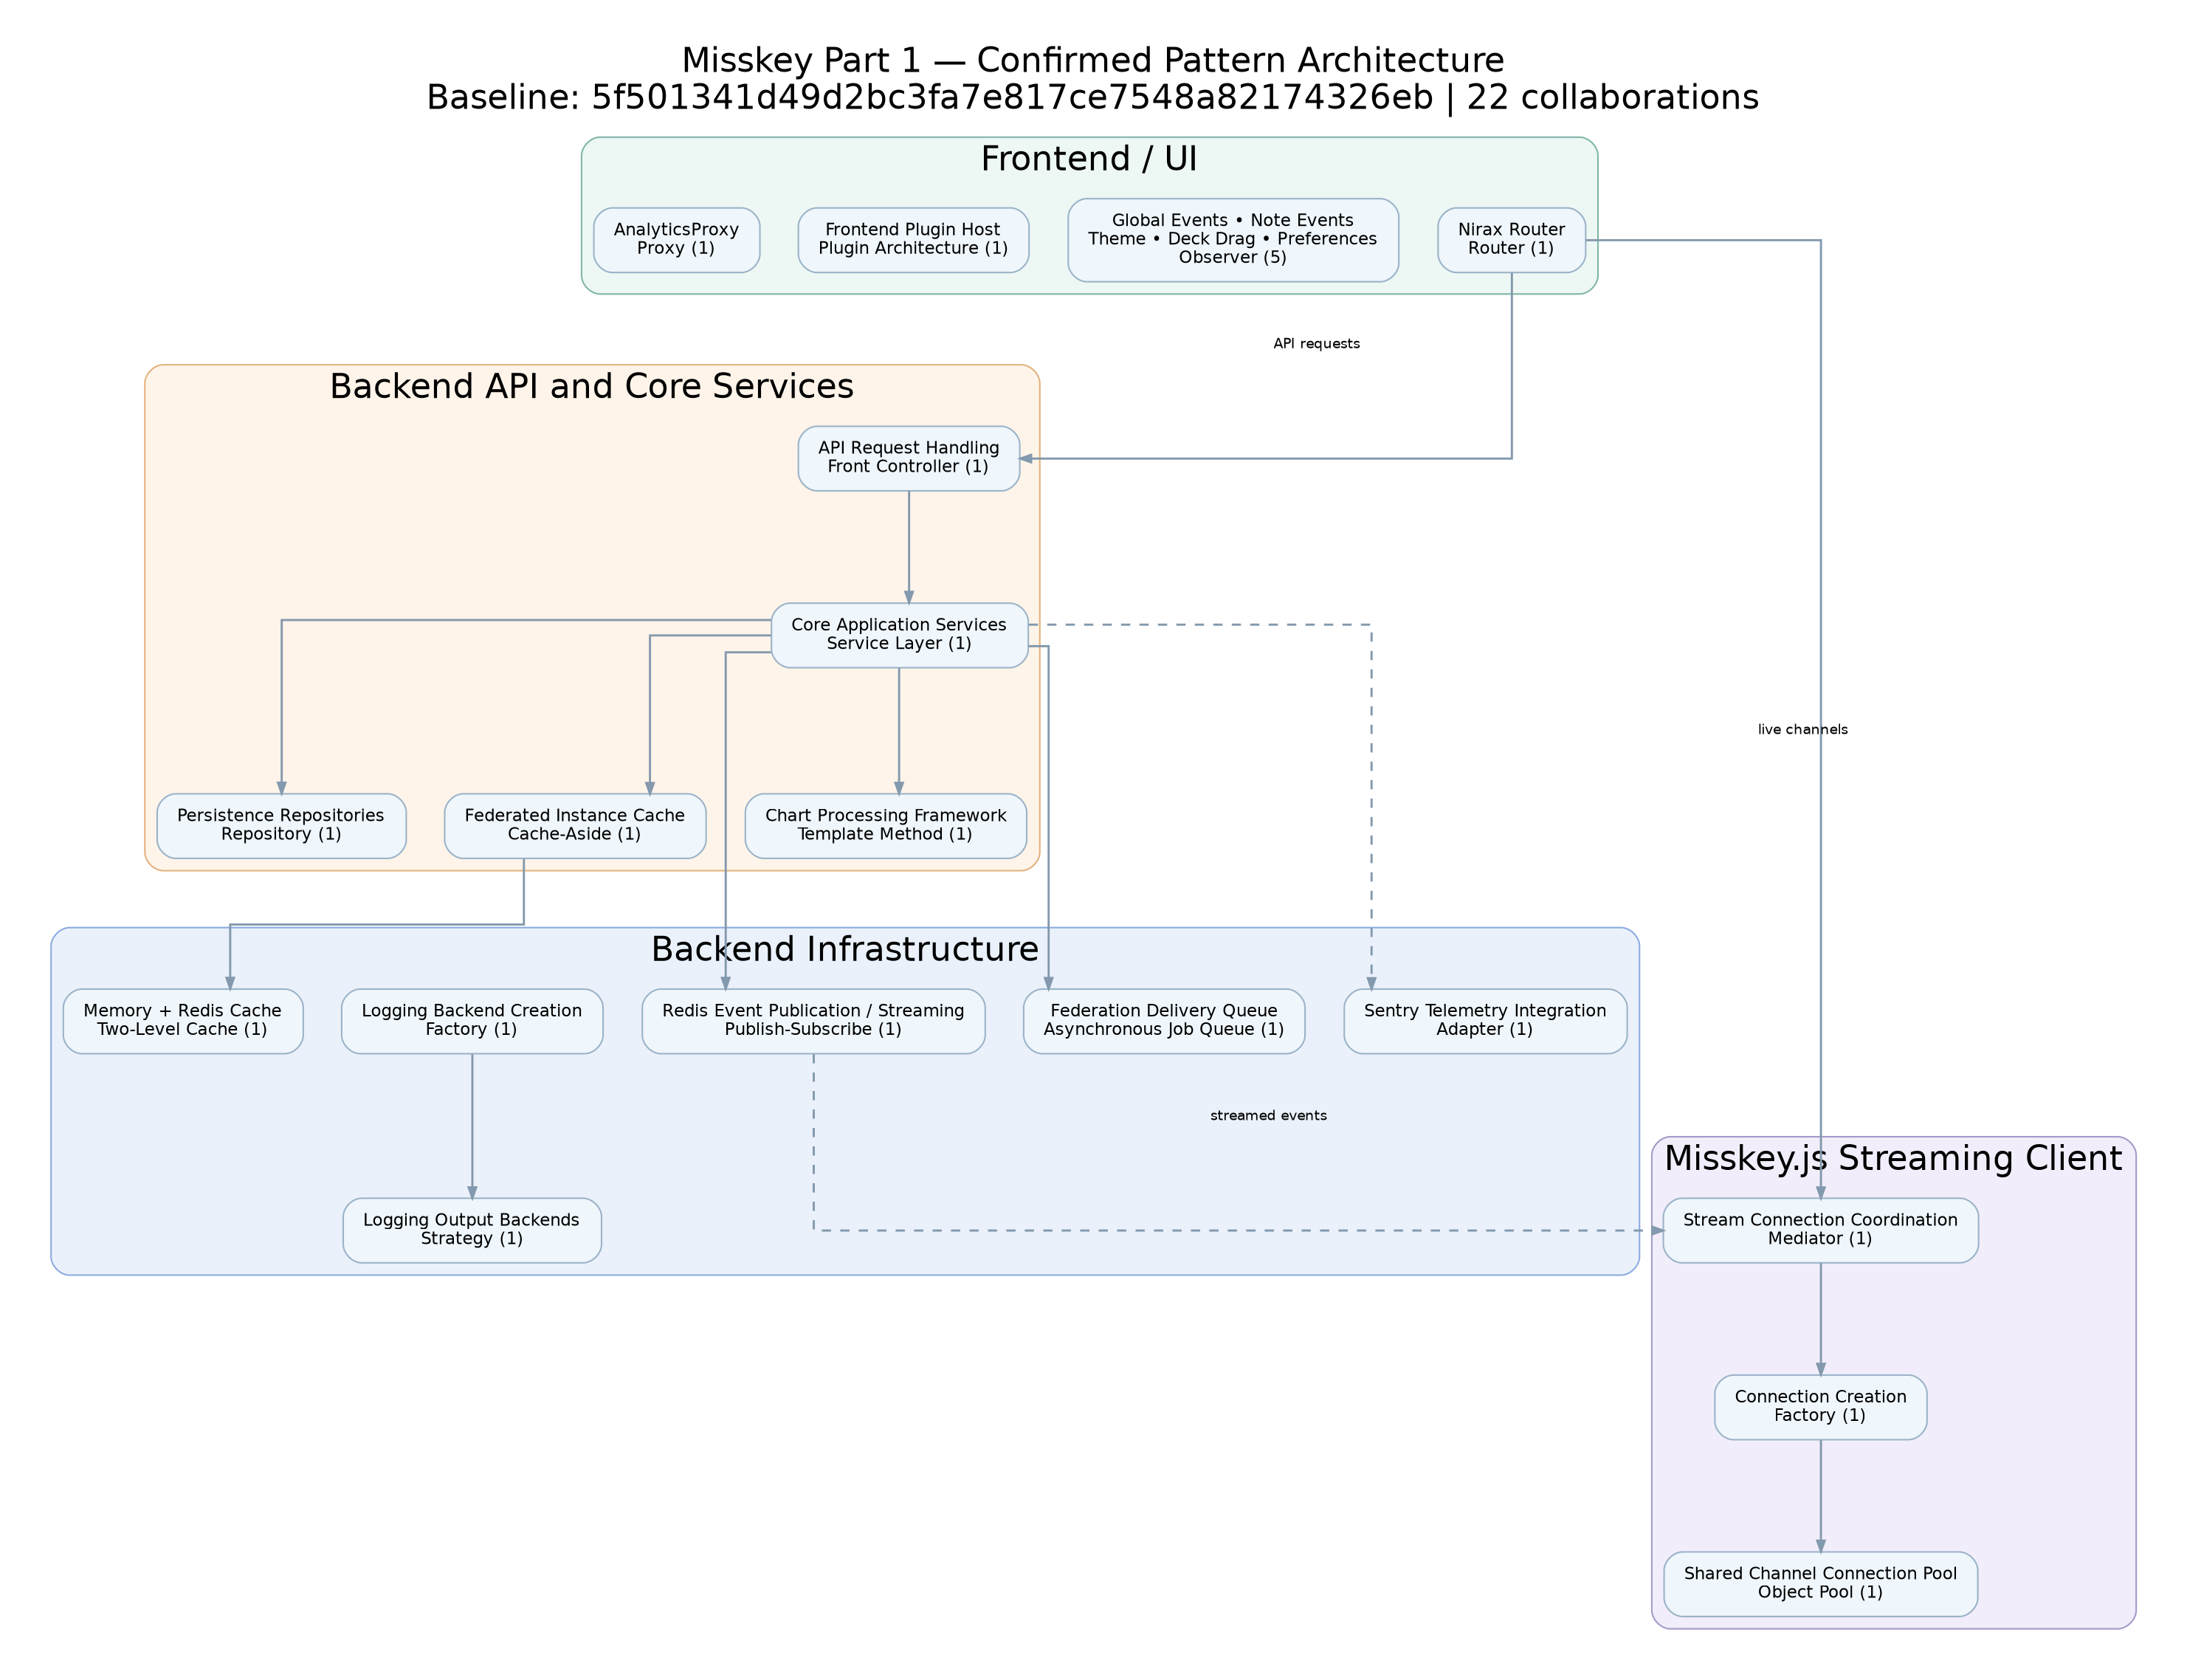
\includegraphics[width=\linewidth]{Part1/pattern_architecture/pattern_architecture.png}\\\small Figure 1: Part 1 pattern architecture (Part1/pattern\_architecture/).\end{center}
\section{Part 1 Pattern discovery}
Method: candidates were found with LLM assistance (ChatGPT, 2026-10-11 per Part1/llm.csv), then classified and retained after source-oriented checks and a missed-pattern scan; the discovery prompt is Part1/Part1\_prompt.txt. Each of the 22 records in Part1/patterns.csv gives participant roles and file/line ranges at the baseline commit.

\subsection{Totals at the baseline}
Confirmed pattern types: 17. Pattern instances recorded: 22. In the Part 3 source re-check three of the 22 (Mediator, Object Pool, Streaming Connection Factory) were rated uncertain, and Repository and the Deck Column Drag Observer needed corrected evidence; Part 3 therefore implemented 15 types (19 certain instances).

\subsection{Pattern inventory}
{\small\begin{tabularx}{\linewidth}{llX}\toprule
Pattern type & Category & Instances\\\midrule
Asynchronous Message Queue / Job Queue & Architectural/Enterprise & 1 \\
Cache-Aside / Lazy Loading & Architectural/Enterprise & 1 \\
Front Controller & Architectural/Enterprise & 1 \\
Plugin Architecture / Microkernel & Architectural/Enterprise & 1 \\
Publish-Subscribe & Architectural/Enterprise & 1 \\
Repository & Architectural/Enterprise & 1 \\
Router & Architectural/Enterprise & 1 \\
Service Layer & Architectural/Enterprise & 1 \\
Two-Level Cache & Architectural/Enterprise & 1 \\
Mediator & Behavioral & 1 \\
Observer & Behavioral & 5 \\
Strategy & Behavioral & 1 \\
Template Method & Behavioral & 1 \\
Factory & Creational & 2 \\
Object Pool / Resource Pooling & Creational & 1 \\
Adapter & Structural & 1 \\
Proxy & Structural & 1\\
\bottomrule\end{tabularx}}

\subsection{Pattern instances}
{\small\begin{tabularx}{\linewidth}{llX}\toprule
\# & Pattern & Instance\\\midrule
1 & Strategy & Logging Output Strategy \\
2 & Adapter & Telemetry Backend Adapter Layer \\
3 & Repository & Misskey Persistence Repository Layer \\
4 & Publish-Subscribe & Global Redis Event Publication and Streaming Subscription \\
5 & Asynchronous Message Queue / Job Queue & Federation Delivery Asynchronous Job Queue \\
6 & Cache-Aside / Lazy Loading & Federated Instance Cache-Aside \\
7 & Two-Level Cache & RedisSingleCache L1/L2 Cache \\
8 & Front Controller & Misskey API Front Controller \\
9 & Factory & Logging Backend Factory \\
10 & Object Pool / Resource Pooling & Misskey.js Shared Streaming Connection Pool \\
11 & Observer & Frontend Global Event Observer \\
12 & Observer & Note-Specific Reactive Event Observer \\
13 & Observer & Theme Manager Observer \\
14 & Observer & Deck Column Drag Observer \\
15 & Mediator & Misskey.js Streaming Connection Coordination \\
16 & Router & Nirax Frontend Router \\
17 & Observer & PreferencesManager Observer \\
18 & Factory & Streaming Connection Factory \\
19 & Service Layer & Misskey Core Application Service Layer \\
20 & Plugin Architecture / Microkernel & Misskey Frontend Plugin Architecture \\
21 & Template Method & Misskey Chart Processing Framework \\
22 & Proxy & AnalyticsProxy\\
\bottomrule\end{tabularx}}

Participant mappings, file paths with line ranges and evidence for every instance are in Part1/patterns.csv (copied to data/patterns.csv).

\section{Part 2 Evolution and refactoring}
Four changes (CH01 to CH04) were implemented on the evolved source in Part2/code; the assignment asks for three. Each change folder in Part2/changes holds the requirement, the diff, the commit record, the test log, metrics.csv and a pattern-effects note; class diagrams are in Part2/diagrams.

{\small\begin{tabularx}{\linewidth}{llllX}\toprule
Change & Feature & Commit & Production LOC before / after & Focused tests\\\midrule
CH01 & Native events with RSVP and reminder notifications & 608b45de20dc & 2704 / 3648 & 21 passed / 21 total (0 failed) \\
CH02 & First-class audio posts with transcription & 9a4398a103e3 & 2834 / 3981 & 21 passed / 21 total (0 failed) \\
CH03 & Context-aware link safety and spam protection & 39e3c987488d & 4350 / 5501 & 29 passed / 29 total (0 failed) \\
CH04 & Explainable, user-controlled personalized feed & b3040278d3e6 & 3391 / 4488 & 20 passed / 20 total (0 failed)\\
\bottomrule\end{tabularx}}

Production LOC was counted with a Python SLOC counter (excluding comments and blanks) over the affected files; CH02 to CH04 are measured against the preceding change, CH01 against the baseline.

\subsection{Updated pattern counts}
{\small\begin{tabularx}{\linewidth}{lllX}\toprule
Snapshot & Pattern types & Pattern instances & Newly introduced\\\midrule
baseline & 11 & 14 & - \\
CH01 & 12 & 15 & State: RSVP Attendance State Machine \\
CH02 & 12 & 17 & Strategy: Audio Transcription Engine Strategies; State: Audio Transcript Lifecycle State Machine \\
CH03 & 12 & 18 & Strategy: Link Reputation Provider Strategies \\
CH04 & 12 & 19 & Strategy: Recommendation Ranking Strategy\\
\bottomrule\end{tabularx}}

Each change reused existing collaborations (dependency injection, repositories, API endpoint factory) and added State and Strategy instances. Refactorings: CH01 introduced an EventReminderSchedule value object (primitive obsession); CH02 replaced status type codes with an AudioTranscriptStateMachine transition table; CH03 centralised URL normalisation and destination validation in LinkSafetyService; CH04 replaced ranking conditionals with Strategy classes. Detail and behaviour-preservation notes are in each Part2/changes/ChangeN/pattern\_effects.md.

\section{Part 3 Cross-language comparison}
One representative verified instance per confirmed pattern type (15 types) was implemented in Java, Python, JavaScript and C++ with shared fixtures: 97 cases, 388 executions, all passing. Detail, tables and references are in Part3/A13\_Part3\_Report.pdf; the data is in data/cross\_language.csv.

{\small\begin{tabularx}{\linewidth}{llllX}\toprule
Language & Median LOC (range) & Max function CC & Median process ms (range) & Tests passed\\\midrule
Java & 37 (22-78) & 9 & 77.1-104.2 & 97/97 \\
Python & 29 (14-61) & 10 & 23.8-55.3 & 97/97 \\
JavaScript & 26 (13-56) & 9 & 43.5-51.0 & 97/97 \\
C++ & 43 (28-92) & 9 & 3.3-3.7 & 97/97\\
\bottomrule\end{tabularx}}

Source LOC and complexity come from lizard; timing is the median of five runs after one warm-up and includes process start-up, so it mostly compares runtime start-up. Four instances are only partly supported by the source (Factory, Front Controller, Service Layer, Repository), and 11 of the 15 are backend code. The Observer oldValue behaviour was reproduced in a stub class, not inside Misskey.

\section{LLM records and human verification}
All records are in data/llm.csv (12 rows). Models: ChatGPT (Part 1), Antigravity Agent (Part 2), Claude Sonnet 5.5 (Part 3). For Part 3, review entries were recorded by Sreehari M (AM.SC.U4CSE23156) on 11/10/2026 (completed with ChatGPT) in Part3/llm/verification/human\_review\_checklist.md: confirmed 1, corrected 4, disputed 2.

{\small\begin{tabularx}{\linewidth}{llX}\toprule
Part & Model and date & Evaluation\\\midrule
Pattern discovery & ChatGPT GPT-6, 2026-10-11 & partial: LLM-assisted candidate discovery and classification \\
Pattern evolution & Antigravity Agent (Google DeepMind) 2026-10-11 & partial: Change 1 implementation fulfilled all acceptance criteria; 21/21 focused tests passed; committed cleanly as 608b45de20dce0a78459025320bfdeb0c \\
Pattern evolution & Antigravity Agent (Google DeepMind) 2026-10-11 & partial: Change 2 implementation fulfilled all acceptance criteria; 21/21 focused tests passed; committed cleanly as 9a4398a103e392a0ea634eaf521470985 \\
Pattern evolution & Antigravity Agent (Google DeepMind) 2026-10-11 & partial: Change 3 implementation fulfilled all acceptance criteria; 29/29 focused tests passed; committed cleanly as 39e3c987488d59045cc3ed5cfe532f6f3 \\
Pattern evolution & Antigravity Agent (Google DeepMind) 2026-10-11 & partial: Change 4 implementation fulfilled all acceptance criteria; 20/20 focused tests passed; committed cleanly as b3040278d3e63cf4ced915f9623b95969 \\
cross-language analysis & Claude Sonnet 5.5 (claude-sonnet-5-5); 2026-10-10 & partial: Counts, commit and cited locations are supported, but the original confidence classifications were too strong for Factory, Front Controller,  \\
cross-language analysis & Claude Sonnet 5.5 (claude-sonnet-5-5); 2026-10-10 & correct: All 60 implementations pass the recorded shared-fixture tests across four languages \\
cross-language analysis & Claude Sonnet 5.5 (claude-sonnet-5-5); 2026-10-10 & partial: The recorded medians, software versions, LOC values and lizard complexity measurements reproduce, but the warm-up timing is not retained in r \\
cross-language analysis & Claude Sonnet 5.5 (claude-sonnet-5-5); 2026-10-10 & correct: The cited source supports the Observer finding and documented corrections \\
cross-language analysis & Claude Sonnet 5.5 (claude-sonnet-5-5); 2026-10-11 & cannot confirm: The supporting scripts and outputs exist, but the verification was produced and checked by the same model family, so it is not indepen \\
cross-language analysis & Claude Sonnet 5.5 (claude-sonnet-5-5); 2026-10-11 & correct: The current slide figures and scope note match the project data and automated deliverable checks \\
cross-language analysis & Claude Sonnet 5.5 (claude-sonnet-5-5); 2026-10-11 & correct: The report tables, counts, scope note and technology discussion align with the project data and automated deliverable checks\\
\bottomrule\end{tabularx}}

Generated code: Part 2 code and tests were produced by the Antigravity agent and committed per change; Part 3 snippets were produced with Claude and corrected after review. Part 1 and Part 2 records do not list a human reviewer.

\section{Findings, contributions and references}
\begin{itemize}
\item The 22 Part 1 records cover 17 pattern types across creational, structural, behavioural and architectural categories.
\item Part 2 added four features without replacing existing collaborations; pattern instances grew from 14 to 19 in the Part 2 counts.
\item All 60 Part 3 implementations pass their shared fixtures; pattern structure is expressed differently per language (nominal interfaces, protocols, duck typing, std::function).
\item Limitations: the Part 1 baseline totals (17 types, 22 instances) and the Part 2 baseline totals (11 types, 14 instances) were produced separately and do not agree; Part 2 has four changes where three were asked; the Part 3 warm-up time was not stored; no LaTeX toolchain was available, so this PDF was generated directly from the report source data.
\end{itemize}
{\small\begin{tabularx}{\linewidth}{llX}\toprule
Roll number & Name & Contribution evidenced in the repository\\\midrule
AM.SC.U4CSE23156 & Sreehari M & Part 3 review entries (checklist section 10) and label updates, commit e9fa6ca \\
AM.SC.U4CSE23148 & Rohit Prasanth & Part 3 cross-language work, records and report \\
AM.SC.U4CSE23157 & Sreyas S Sankar & Part 1 pattern discovery files (commits from account SR3YAS237) \\
AM.SC.U4CSE23173 & Sreevisakh A & Part 2: native events and audio transcription (CH01, CH02), per CONTRIBUTOR\_S-visakh.md \\
AM.SC.U4CSE23168 & Vighnesh H & Part 2 changes and evolved source (commits from account vighnesh1001)\\
\bottomrule\end{tabularx}}

References: Misskey source (https://github.com/misskey-dev/misskey), commits 5f501341, 608b45de, 9a4398a1, 39e3c987, b3040278; Python typing documentation (https://docs.python.org/3/library/typing.html); Node.js Events (https://nodejs.org/api/events.html); cppreference std::function; Java Language Specification SE 17, chapter 9; radon and lizard documentation. Part 3 references are listed in Part3/A13\_Part3\_Report.pdf.

\end{document}
